\section{سوال دوم}
در این سوال برای از الگوریتم ابتکاری مورچگان برای حل مسئله معروف فروشنده دوره‌گرد استفاده شده است. در بخش
\ref{sec:part_I}
با فرض نبودن ترافیک،
در بخش
\ref{sec:part_II}
با فرض ترافیک و در بخش
\ref{sec:part_III}
با فرض اینکه ترافیک تابعی از زمان است حل شده است. در شکل
\ref{fig:cities}
مکان شهر‌ها رسم شده است.
\begin{figure}[H]\label{fig:cities}
	\caption{مکان شهرها} 
	\centering 
	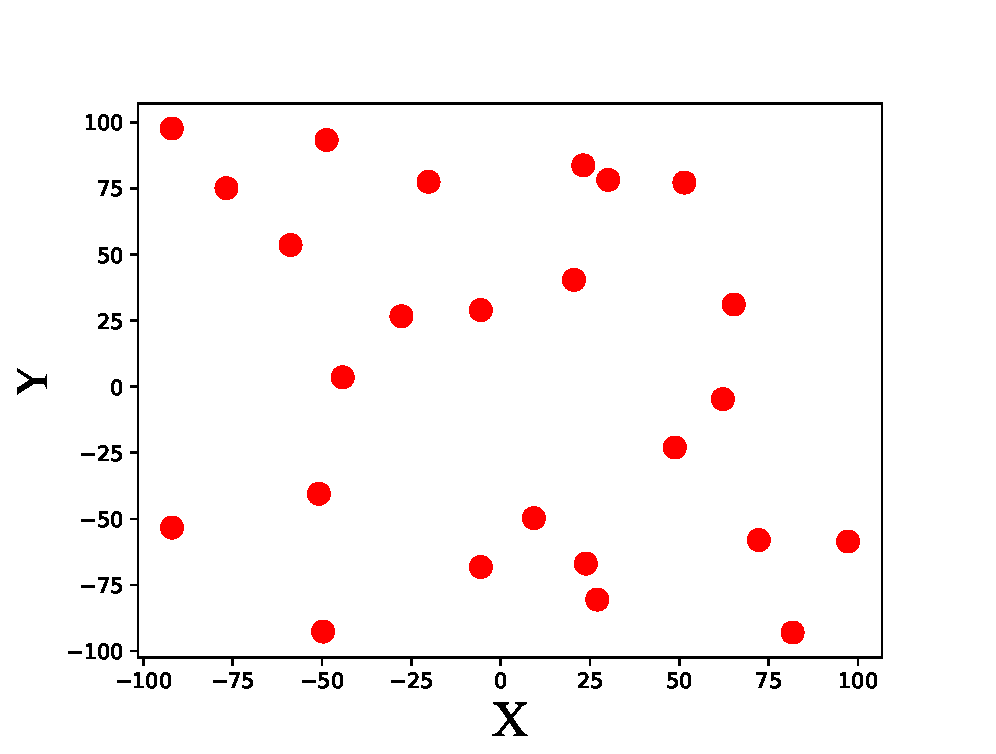
\includegraphics[width=16cm]{../Figure/Q2/Cities} 
\end{figure}
\subsection{پخش اول}\label{sec:part_I}
با توجه به اینکه الگوریتم مورد استفاده ابتکاری است و تابع رندوم بخش مهمی از آن است در اینجا دو راه حل (شکل های
\ref{fig:part_I_ACO_sol_1}
و 
\ref{fig:part_I_ACO_sol_2}
) آورده شده است. طول هر مسیر نیز در جدول \ref{tab:part_I_cost}
آورده شده است. برای حل این مسئله از یک ماتریس به اسم
\lr{graph}
 برای توصیف فاصله‌ی بین شهرها استفاده شده است

\begin{figure}[H]\label{fig:part_I_ACO_sol_1}
	\caption{راه حل اول تولید شده توسط الگوریتم ACO} 
	\centering 
	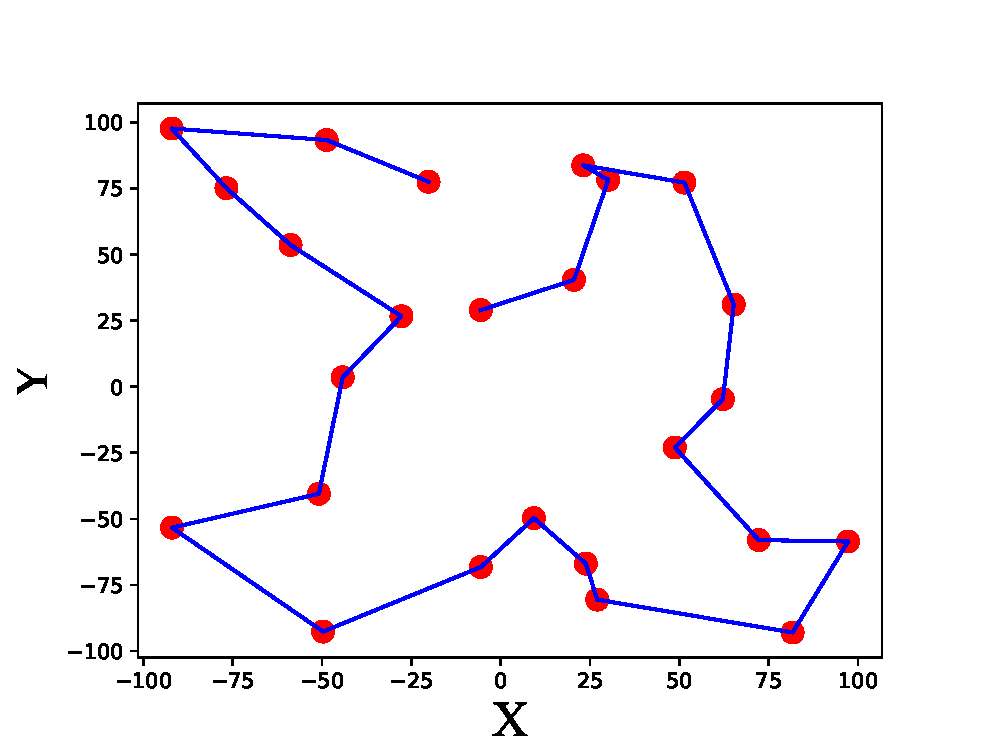
\includegraphics[width=16cm]{../Figure/Q2/ACO_solution} 
\end{figure}

\begin{figure}[H]\label{fig:part_I_ACO_sol_2}
	\caption{راه حل دوم تولید شده توسط الگوریتم ACO} 
	\centering 
	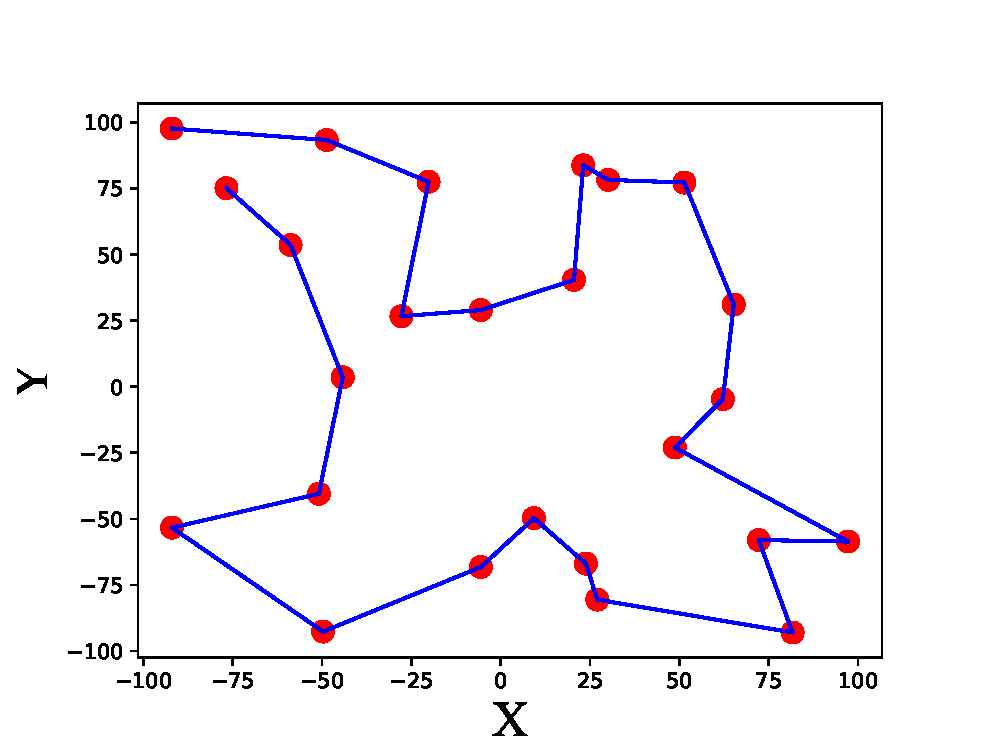
\includegraphics[width=16cm]{../Figure/Q2/ACO_solution_1} 
\end{figure}

\lr{\begin{table}[H]\label{tab:part_I_cost}
		\caption{Cost of solution produced with ACO}
		\vspace{0.5cm}
		\centering
		\begin{tabular}{|c|c|c|}
			\hline
			\lr{solution 2 Cost} & \lr{solution 1 Cost}\\
			\hline
			899.8 & 881.0\\
			\hline
		\end{tabular}
\end{table}}

\subsection{بخش دوم}\label{sec:part_II}

در بخش
\ref{sec:part_I}
ماتریس
\lr{graph}
معرفی شد. در این بخش برای اضافه کردن ترافیک، درایه‌های ماتریس
\lr{traffic}
به‌صورت نظیر به نظیر تقسیم بر درایه‌های ماتریس
\lr{graph}
(هر چه سرعت بیشتر باشد هزینه رفتن از شهر i به j کمتر است) می‌شود.

\begin{figure}[H]
	\caption{راه حل تولید شده توسط الگوریتم ACO با در نظر گرفتن ترافیک} 
	\centering 
	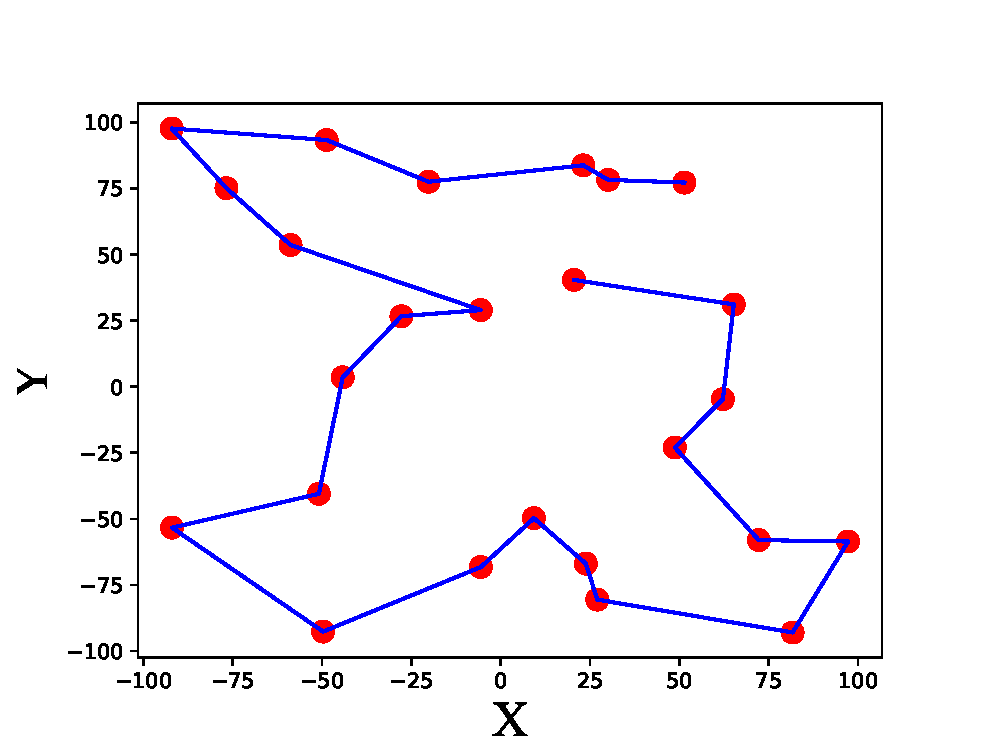
\includegraphics[width=16cm]{../Figure/Q2/ACO_traffic_solution} 
\end{figure}

\subsection{بخش سوم}\label{sec:part_III}

\lr{\begin{table}[H]\label{tab:part_III_cost}
		\caption{Cost of solution produced with ACO}
		\vspace{0.5cm}
		\centering
		\begin{tabular}{|c|c|c|}
			\hline
			\lr{global pheromone solution} & \lr{local pheromone solution} & \lr{Time}\\
			\hline
			879.96 & 874.72& \lr{i = 0}\\
			1571.60 & 1491.50& \lr{i = 1}\\
			1138.58 & 936.80& \lr{i = 2}\\
			1152.92 & 1130.20& \lr{i = 3}\\
			1095.87 & 1011.32& \lr{i = 4}\\
			1080.46 & 1030.46& \lr{i = 5}\\
			1357.68 & 1324.29& \lr{i = 6}\\
			1077.28 & 1081.62& \lr{i = 7}\\
			1163.53 & 1129.28& \lr{i = 8}\\
			1309.49 & 1329.87& \lr{i = 9}\\
			\hline
			11827.44 & 11340.11 & sum\\
			\hline
		\end{tabular}
\end{table}}



